\documentclass{article}
\usepackage[utf8]{inputenc}

% Author: Coenrad Fourie
% Last modification: 21 April 2021

\title{\Large{Electronics 315}
\Large{\centerline{\textbf{Practical 3 Report}}}
\large{\centerline{\textbf{Class-AB power amplifier with preamplifier}}}
}
\author{\large{\textbf{Name:} Coenrad Fourie}
\large{\centerline{\textbf{Student Number:} 12345679}}}
\date{4 June 2021}

\usepackage{natbib}
\usepackage{graphicx}
\usepackage{siunitx}
\usepackage{multicol}
\usepackage{xcolor}
\usepackage{geometry}
 \geometry{
 a4paper,
 total={170mm,257mm},
 left=20mm,
 top=20mm,
 }

\begin{document}

\maketitle
\setlength{\parindent}{0pt}
\setlength{\parskip}{1em}

\section{Plagiarism Declaration}
By submitting this assignment with your name and student number filled in you agree with the following statements:

\textit{"I have read and understand the Stellenbosch University Policy on Plagiarism and the definitions of plagiarism and self-plagiarism contained in the Policy [Plagiarism: The use of the ideas or material of others without acknowledgement, or the re-use of one’s own previously evaluated or published material without acknowledgement or indication thereof (self-plagiarism or textrecycling)]."}

\textit{"I know that plagiarism is a punishable offence and may be referred to the University's Central Disciplinary Committee (CDC) who has the authority to expel me for such an offence."}

\textit{"I declare that, except where a source has been cited, the work contained in this assignment is my own work and that I have not previously (in its entirety or in part) submitted it for grading in this module/assignment or another module/assignment."}

\hrule

% Cut this out (below)
--------------  Cut this out --------------- $\downarrow$

\textcolor{red}{THIS REPORT COUNTS FOR A TOTAL OF 10 MARKS AND MAKES UP ONE THIRD OF THE OVERALL GRADE FOR THE PRACTICAL. TO GET THE MARKS FOR A SECTION, THE CONTENT MUST BE COMPLETE, COMPREHENSIVE AND MATCH THE RESULTS OBTAINED FROM THE SIMULATION TEST BENCH AND THE PRACTICAL DEMONSTRATION. IF ANY SECTION IS OMITTED, THE REPORT CANNOT SCORE HIGHER THAN 4/10.}

--------------  Cut this out --------------- $\uparrow$
% Cut this out (above)


% -------------------------------------------------------------------------------------------------------------------
% -------------------------------------------------------------------------------------------------------------------
\section{Circuit Diagram}
\textbf{This section counts for 1 mark.}

This section should contain a complete circuit diagram for your design (both preamplifier and power amplifier stages must be included). Label the components in the diagram so that you can easily refer to them throughout the rest of the report.

\begin{figure}[h!]
  \centering
  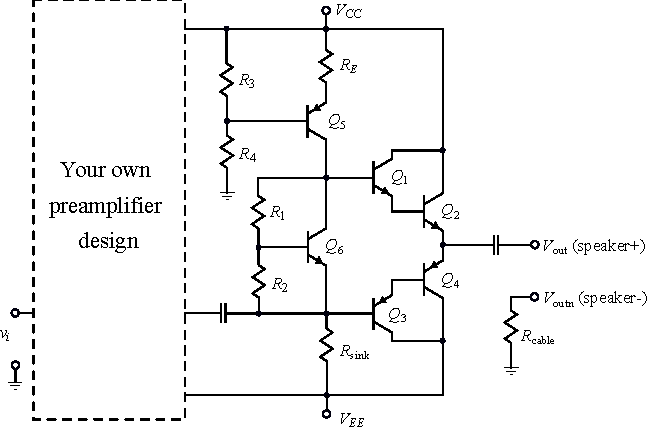
\includegraphics[width=0.6\linewidth]{images/circdiagram.pdf}
  \caption{Circuit diagram of amplifier.}
  \label{fig:circschem}
\end{figure}


% -------------------------------------------------------------------------------------------------------------------
% -------------------------------------------------------------------------------------------------------------------
\section{Power Amplifier Design}
\textbf{This section counts for 2 marks.}

This section should include a detailed description of the entire design process for the power amplifier stage. All equations should be included. All design decisions should be substantiated. Discuss any fine-tuning to theoretical values that may have been performed as a result of initial simulations.

% -------------------------------------------------------------------------------------------------------------------
% -------------------------------------------------------------------------------------------------------------------
\section{Preamplifier Design}
\textbf{This section counts for 1 mark.}

This section should include a detailed description of the entire design process for the preamplifier stage. All equations should be included. All design decisions should be substantiated. Discuss any fine-tuning to theoretical values that may have been performed as a result of initial simulations.


% -------------------------------------------------------------------------------------------------------------------
% -------------------------------------------------------------------------------------------------------------------
\section{Frequency Analysis and Capacitor Design}
\textbf{This section counts for 1 mark.}

This section should include a description of the steps taken to perform a frequency analysis and choose the capacitor values in your design. (i.e. choice of capacitor for dominant pole, frequencies designed for, equations used, etc.). Also discuss any fine-tuning to theoretical capacitor values that may have been performed as a result of initial simulations.


% -------------------------------------------------------------------------------------------------------------------
% -------------------------------------------------------------------------------------------------------------------
\section{Power and Thermal Analysis}
\textbf{This section counts for 2 marks -- 1 for power analysis and any relevant discussion and 1 for thermal analysis and any relevant discussion.}

This section should include a list of the power dissipated in every component of the amplifier system. Detail the equations used to calculate power dissipation in the transistors and to perform a thermal analysis (example shown below). Include a discussion of steps taken (if any) to account for high power dissipation in specific components or an unsatisfactory thermal response for transistors.


\begin{equation} \label{eqn:pwr}
  P_{Q1} = V_{CE}I_{C} = 
\end{equation}

\begin{equation} \label{eqn:temp1}
  T_{j1} = \left(\theta_{jc}+\theta_{ca}\right)P_{Q1} = 
\end{equation}


\begin{table}[!htbp]
\centering
\begin{tabular}{ c | c } 
\hline
\textbf{COMPONENT} & \textbf{POWER DISSIPATION} \\
\hline
R1  &  \SI{4.54}{\milli\watt} \\
R2  &  \SI{0.9}{\watt} \\
Q1  &  \SI{278}{\milli\watt} \\
\hline
\end{tabular}
\caption{Power dissipation of components.}
\label{table:pwrdissipation}
\end{table}

% -------------------------------------------------------------------------------------------------------------------
% -------------------------------------------------------------------------------------------------------------------
\section{Results and Conclusions}
\textbf{This section counts for 2 marks.}

This section should include a discussion of the results obtained using the SPICE test bench with your design and the measurements of the physical circuit. Shortfalls and potential improvements to your design should be included here.



\end{document}


